%!TEX TS-program = xelatex
\documentclass[9pt]{beamer}

\usepackage{HSE-theme/beamerthemeHSE} % Подгружаем тему

%%% Работа с русским языком и шрифтами
\usepackage[english,russian]{babel}   % загружает пакет многоязыковой вёрстки
\usepackage{fontspec}      % подготавливает загрузку шрифтов Open Type, True Type и др.
\defaultfontfeatures{Ligatures={TeX},Renderer=Basic}  % свойства шрифтов по умолчанию
\setmainfont[Ligatures={TeX,Historic}]{Arial} %  установите шрифты Myriad Pro или (при невозможности) замените здесь на другой шрифт, который есть в системе — например, Arial
\setsansfont{Arial}  %  установите шрифты Myriad Pro или (при невозможности) замените здесь на другой шрифт, который есть в системе — например, Arial
\setmonofont{Courier New}
\uselanguage{russian}
\languagepath{russian}
\usepackage[export]{adjustbox}
\newcommand{\lsum}{\sum\limits}
\usepackage{wrapfig}
\deftranslation[to=russian]{Theorem}{Теорема}
\deftranslation[to=russian]{Definition}{Определение}
\deftranslation[to=russian]{Definitions}{Определения}
\deftranslation[to=russian]{Corollary}{Следствие}
\deftranslation[to=russian]{Fact}{Факт}
\deftranslation[to=russian]{Example}{Пример}
\deftranslation[to=russian]{Examples}{Примеры}

\renewcommand{\thefootnote}{\fnsymbol{footnote}}

\usepackage{lipsum}
\newcommand\Fontvi{\fontsize{6}{7.2}\selectfont}
\newcommand\Fontvj{\fontsize{8}{7.2}\selectfont}

\usepackage[weather]{ifsym}

\usepackage{graphicx}
\usepackage{caption}
\usepackage{subcaption}

\usepackage{multicol} 		% Несколько колонок
\graphicspath{{images/}}  	% Папка с картинками
\usepackage{lscape}
\usepackage{sidecap}
\usepackage{booktabs}
\usepackage{multirow}


%%% Информация авторе и выступлении
\title[Заголовок]{Анализ устойчивости платежного баланса Российской Федерации с помощью модели внешнеэкономической деятельности} 

\author[Карпова Анастасия, БЭК165]{Карпова Анастасия\\
	 БЭК165 \\ \smallskip \scriptsize \url{asyakarpovaa@gmail.com}}

\institute[Высшая школа экономики]{Научный руководитель: Ужегов А.А. \\ \vspace{4ex}  Национальный исследовательский университет \\ «Высшая школа экономики» (Москва)}
\date{1 июня 2020 г.}

\begin{document}	% Начало презентации

\frame[plain]{\titlepage}	% Титульный слайд



\begin{frame}
\frametitle{Цели и задачи}

\textbf{Цель:} модельно описать внешнеэкономическую деятельность РФ для построения сценарных прогнозов основных компонент платежного баланса, валютного курса, показателей топливных рынков и покупки валюты в рамках бюджетного правила.

\vspace{4ex}

\textbf{Задачи}:
\begin{itemize}
\item Обзор способов моделирования внешнеэкономической деятельности;
\item Сбор и обработка статистических данных;
\item Построение модели и ее программная реализация на языке R;
\item Построение месячных прогнозов основных переменных модели на краткосрочный период (1 год);
\item Анализ устойчивости\footnote[1]{Под устойчивостью в работе понимается способность поддержания положительного сальдо счета текущих операций.} платежного баланса при различных сценариях с помощью построенной модели.
\end{itemize}

\end{frame}


\begin{frame}
\frametitle{Обзор литературы}
\framesubtitle{Подходы к моделированию внешнеэкономической деятельности}


\begin{itemize}
	\item \textbf{Модели малой открытой экономики с платежным балансом} 
	
	Моделируется поведение фирм, домохозяйств, монетарных и фискальных властей.
	В ходе численного решения находится равновесное значение платежного баланса (Mendoza E., Uribe M., 1999).
	
	\item \textbf{Стохастические модели общего равновесия (DSGE)}
	
	Более гибкие при моделировании поведения агентов. 
	Позволяют проводить симуляции экономики и строить функции импульсного отклика для анализа шоков (Cubas, G., 2011).
\end{itemize}

	\textit{Особенности}: моделирование нескольких агентов; теоретические предпосылки о связи переменных и особенностях поведения агентов.	
	
	\begin{itemize}
	\item \textbf{Статистические модели}
	
	Основаны на статистическом исследовании динамики временных рядов.
	Позволяют анализировать взаимосвязи переменных и находить предикторы, полезные для прогнозирования других рядов (Freund, 2005).
\end{itemize}	

\textit{Особенности}: базовые теоретические предпосылки о связях переменных; основная трудность в подборе предикторов и обработке данных; более простая процедура построения и оценки моделей.
\end{frame}

\begin{frame}
	\frametitle{Данные}
	\begin{itemize}
		\item Фактические данные, используемые в модели, покрывают период с первого
		квартала 2006 года по первый квартал 2020 года.
		
		\item Квартальные данные по всем рядам доступны за весь рассматриваемый период.
		Месячные данные по некоторым рядам отсутствуют на протяжении нескольких лет.
		
		
	\end{itemize}	
	\begin{center}
		\small
		\begin{tabular}{ l | c }
			\toprule
			Данные  &  Источник  \\
			\midrule
			переменные платежного баланса & ЦБ РФ \\ 
			\midrule
			ключевая ставка & ЦБ РФ \\
			\midrule
			цена Brent и природного газа & World Bank Commodity Price Data \\
			\midrule	
			покупка валюты & Минфин\\
			\midrule
			ВВП и его компоненты & Росстат\\
			\midrule
			доходность 10Y Treasury & Investing.com\\
			\bottomrule			
		\end{tabular}
		\captionof{table}{Источники данных}\label{tab:7} 
		\normalsize
	\end{center}
	
\end{frame}

\begin{frame}
\frametitle{Модель внешнеэкономической деятельности РФ}
\begin{itemize}
\item Модель развивает идеи статьи Пильник $\&$ Ужегов, 2017.
Основная часть модели посвящена платежному балансу.
\item Состоит из набора эконометрических и балансовых соотношений, оцениваемых в системе либо по отдельности.
\item Модель включает набор экзогенных переменных, динамика которых не объясняется, но используется для прогнозирования и сценарного анализа.
\item Для России, как экспортно - ориентированной экономики, торговый баланс формирует основную часть счета текущих операций, поэтому предполагается связь динамики платежного баланса и валютного курса, а также объема продажи валюты в рамках бюджетного правила.

%%% картинка про структуру экспорта
\end{itemize}
	%\begin{figure}
	%	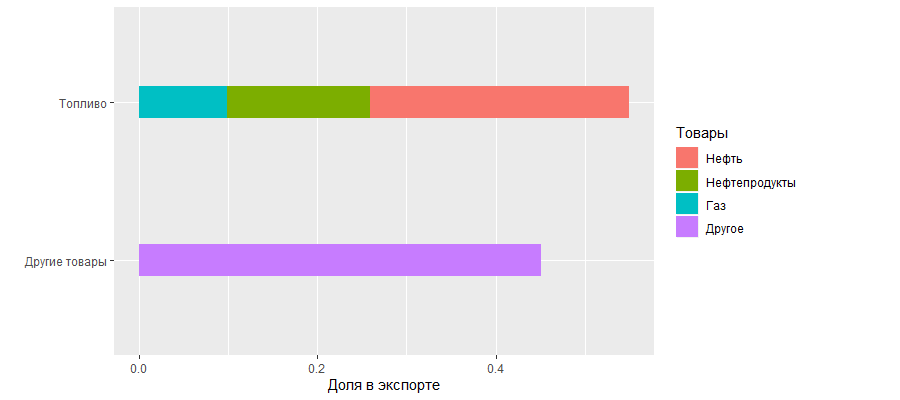
\includegraphics[width=7cm]{export_structure.png}
	%	\caption{Структура экспорта РФ, 2019 год}\label{fi:1}
	%	\captionsetup{justification=centering,margin=0.8cm}
		%%	\caption*{Доля нефти, нефтепродуктов и газа в экспорте РФ в 2019 году составила $55\%$. 
		%%		Для каждого из ресурсов строится отдельная модель.}
	%\end{figure}

\begin{landscape}
	\vspace*{-0.2cm}
	\hspace*{0.5cm}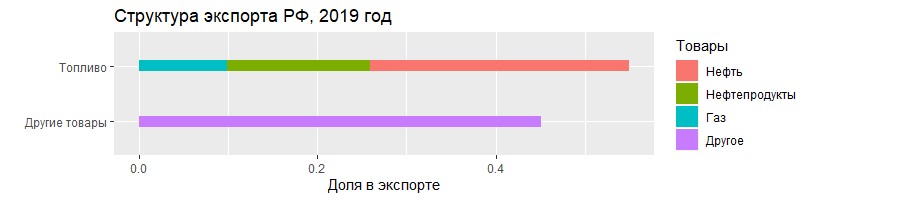
\includegraphics[width = 12 cm]{1.png}\hspace*{-1cm}
\end{landscape}

\end{frame}

\begin{frame}
	\frametitle{Структура модели}
	\begin{center}
	\small
	\begin{tabular}{ l | c }
		\toprule
		Эндогенные переменные  &  Обозначение в модели  \\
		\midrule
		\multicolumn{2}{c}{\textbf{модель платежного баланса}} \\
		\midrule
		\multicolumn{2}{c}{\textbf{модели топливных ресурсов}\footnote[1]{в рамках модели оцениваются отдельные системы для нефти, газа и нефтепродуктов}}\\
		\midrule
		средняя цена экспорта ресурса & \textit{ p\_exp\_oil } \\ 
		объем экспорта ресурса & \textit{ v\_exp\_oil } \\
		выручка от экспорта &  \textit{ r\_exp\_oil } \\ 
		\midrule
		\textbf{валютный курс (USD/RUB)} & \textit{ rub\_usd } \\ 
		\midrule
		\textbf{покупка валюты по бюджетному правилу} & \textit{ r\_cur\_purch } \\ 
		\bottomrule
	\end{tabular}
	\captionof{table}{Блоки модели}\label{tab:1} 
\end{center}
\end{frame}

\begin{frame}
	\frametitle{Моделирование платежного баланса}
	Оценивается несколько систем уравнений.
	
	\begin{center}
		\small
		\begin{tabular}{l | l | c }
			\toprule
			№ & Система  &  Уравнения  \\
			\midrule
			1 & Экспорт (1) & экспорт товаров, экспорт других товаров \\ 
			\midrule
			2 & Экспорт (2) & экспорт услуг, торговый баланс, баланс услуг \\
			\midrule
			3 & Импорт & импорт товаров, импорт услуг, совокупный импорт \\
			\midrule
			5 &  & баланс оплаты труда \\
			\midrule
			6 &  & баланс вторичных доходов \\
			\midrule
			7 & Баланс инвест. доходов & баланс инвест. доходов, счет текущих операций \\
			\midrule
			8 &  & изменение резервных активов \\
			\midrule
			9 &  & чистые пропуски и ошибки \\
			\bottomrule			
		\end{tabular}
		\captionof{table}{Платежный баланс: системы и уравнения}\label{tab:8} 
		\normalsize
	\end{center}

	\textbf{Финансовый баланс}	
			\[
	\widehat{\text{r\_bal\_fin}}_t = \widehat{\text{r\_cur\_acc}}_t + \widehat{\text{r\_errors}}_t - \widehat{\text{dif\_res}}_t
	\]
	
\end{frame}

\begin{frame}
		\frametitle{Особенности моделирования платежного баланса}
			\begin{figure}[htp!]
			\centering
			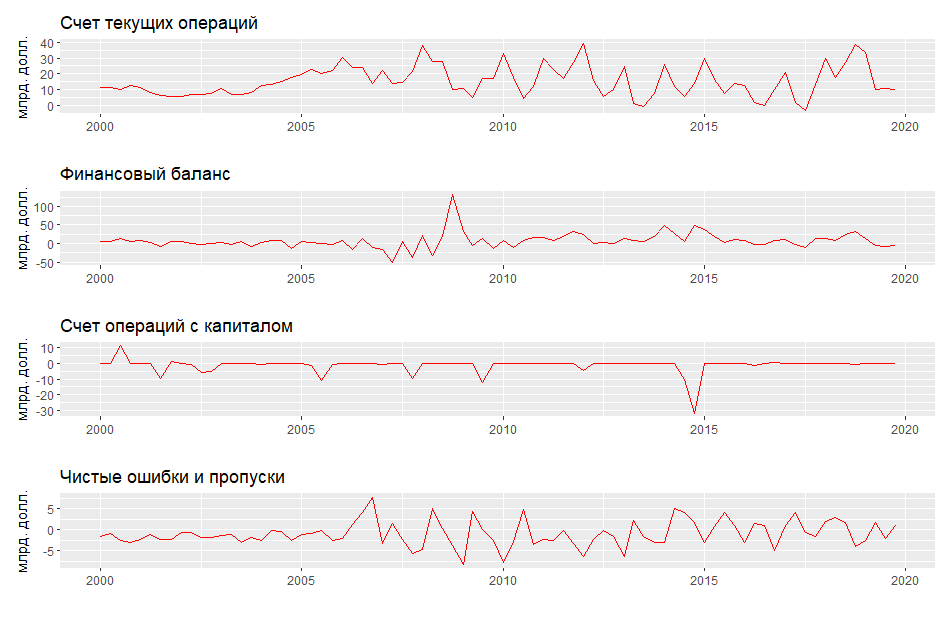
\includegraphics[width=\textwidth]{struct.png}
			\captionsetup{justification=centering}
			\caption{Структура платежного баланса}
		\end{figure}
\end{frame}


\begin{frame}
	\frametitle{Модель топливных ресурсов (нефть)}
Типичная система модели на примере блока нефти:

\begin{align*} 
\small
	\begin{cases}
	\text{p\_exp\_oil}_t =&c_1 + c_2 \cdot \text{brent}_{t-1} + c_3 \cdot \text{brent}_{t-3} + \varepsilon_{t,p}\\
	\text{v\_exp\_oil}_t =&\lsum_{j = 1}^{11} d_j \cdot \text{dum}_{jt} \cdot(a_1 + a_2 \cdot \text{v\_exp\_oil}_{t-3} + a_3 \cdot \text{usd\_rub}_{t-1} + \\ 
	&+ \quad a_4 \cdot \text{p\_exp\_oil}_{t-3}) + \varepsilon_{t,v}\\
	\text{r\_exp\_oil}_t =&\text{p\_exp\_oil}_t \cdot \text{v\_exp\_oil}_t + \varepsilon_{t,r},
	\end{cases}
\end{align*}

где уравнения на цену и объем нефти — пример эконометрических соотношений, а выручка — балансовое соотношение (должно быть выполнено по определению: $\text{выручка} = \text{цена} \times \text{объем}$).
\end{frame}

\begin{frame}
	\frametitle{Моделирование изменения резервных активов}
	
	С помощью подбора предикторов можно учитывать смену режима монетарной политики.
	
\begin{align*}
\footnotesize
\begin{cases}
\text{dif\_reserves}_t &= c_1 + c_2 \cdot \widehat{\text{dif\_reserves}}_{t-1} + \lsum_{j = 1}^{11} d_j \cdot \text{dum}_{jt} + \\
& + \quad c_3 \cdot \widehat{\text{r\_cur\_acc}}_{t} + c_4 \cdot \widehat{\text{r\_cur\_acc}}_{t-1} + \\
& + \quad \left(c_5 + c_6 \cdot \frac{\text{vcor}_t}{\text{usd\_rub}_{t-1}}\right) \cdot \Delta \text{brent}_t + \\
&+ \quad c_7 \cdot \Delta \text{usd\_rub\_}_t + c_8 \cdot \Delta \text{usd\_rub}_{t-1} + c_9 \cdot \Delta \text{usd\_eur}_{t}+ \varepsilon_{t, df_{1}}\\ 
\text{dif\_reserves2}_t &= a_1 + a_2 \cdot \widehat{\text{dif\_reserves}}_{t-1} + \lsum_{j = 1}^{11} f_j \cdot \text{dum}_{jt} + \\
&+ \quad a_3 \cdot \widehat{\text{r\_cur\_acc}}_{t} + a_4 \cdot \widehat{\text{r\_cur\_acc}}_{t-1} + a_5 \cdot \Delta \text{brent}_t + \\
&+ \quad a_6 \cdot \Delta \text{usd\_rub\_}_t + a_7 \cdot \Delta \text{usd\_rub\_}_{t-1} + a_8 \cdot \Delta \text{usd\_eur}_{t} + \\
&+ \quad a_9 \cdot \widehat{\text{r\_cur\_purch}}_t +  a_{10} \cdot \widehat{\text{r\_cur\_purch}}_{t-1} + \varepsilon_{t, df_{2}}, \\ 
\end{cases}
\end{align*}		
	где первое уравнение содержит переменную ширины валютного коридора $\text{vcor}_t$, а второе —  переменную покупки валюты $\text{r\_cur\_purch}_t$.
	Первое уравнение предназначено для восстановления динамики ряда до конца $2014$ года.
\end{frame}

\begin{frame}
	\frametitle{Моделирование валютного курса}
\begin{itemize}
	\item На первом шаге оценивается уравнение на прирост величины валютного курса $\text{rub\_usd\_growth}_{t}$:
\footnotesize
\begin{align*}
\text{rub\_usd\_}&\text{growth}_{t} = c_1 + c_2 \cdot \text{rub\_usd\_growth}_{t-1} + c_3 \cdot \text{usd\_eur\_ratio}_{t} + \\
& + \quad \left(c_4 + c_5 \cdot \text{dum\_1114}_t + c_6 \cdot \frac{\text{vcor}_t}{\text{usd\_rub}_{t-1}}\right)\cdot \text{brent\_ratio}_t + \\
&  + \quad (c_7  + c_8 \cdot \text{dum\_1114}_t)\cdot \text{em\_index\_ratio}_t + \\   
& + \quad c_9 \cdot \text{dif\_r}_t \cdot \text{dum\_1114}_t + 
\lsum_{i = 0, 1} c_{10+i}\cdot\text{r\_cur\_purch}_{t-i} + \varepsilon_{t}
\end{align*}
\normalsize
\item На втором шаге на основании полученного прогноза прироста строится несколько прогнозов валютного курса с разной стартовой точкой с шагом в квартал (с июня 2006 г., с сентября 2006 г. и т.д.)
\item Итоговый прогноз валютного курса получается путем усреднения в каждой точке прогнозов, полученных на втором шаге.

\end{itemize}
\end{frame}


\begin{frame}
	\frametitle{Процедура оценки}
\begin{itemize}
	\item Смысл \textbf{целевой функции} — учесть при подборе коэффициентов ошибку как на месячных, так и на квартальных значениях:
	\[
	E(y_m, \hat y_m, y_q, \hat y_q; \alpha) = || y_m - \hat y_m ||_2 + \alpha|| y_q - \hat y_q ||_2,
	\]
	где $y_m$ — фактические месячные значения временного ряда, $\hat y_m$ — восстановленные моделью значения этого ряда, $y_q$ — фактические квартальные значения, $\hat y_q$ — восстановленные квартальные значения, $\alpha$ — параметр регуляризации.
	
	
\end{itemize}

\end{frame}

\begin{frame}
	\frametitle{Результаты модели}
	\begin{itemize}
		\item Для сравнения моделей данные поделены на две части: обучающая выборка — до $2018$ года, тестовая выборка — $2019$ год.
		
		\item В качестве бенчмарков выбраны ARIMA, ets и сезонный
		наивный прогноз.
		
		\item Модели сравнивались по двум метрикам: MAPE и MASE.
		
		\footnotesize
		
		\[
		MAPE = \frac{1}{n}\sum_{t=1}^{n}\left|\frac{Y_t - \hat Y_t}{Y_t}\right|,
		\]
		
		\[
		MASE = \frac{\frac{1}{J} \sum_j |e_j|}{\frac{1}{T-1} \sum_{t=2}^T|Y_t - Y_{t-1}|},
		\]
		\normalsize
		
		\item Прогнозная сила модели внешнеэкономической деятельности оказалась выше для $18$ переменных из $27$ по MAPE и для $12$ переменных из $27$ по MASE.
	\end{itemize}

где $Y_t$ — фактические значения ряда, $\hat Y_t$ — прогноз, $n$ — длина прогноза, $J$ — длина тестовой выборки, $T$ — длина обучающей выборки, $e_t$ — ошибка прогноза исследуемой модели.

\end{frame}

\begin{frame}
	\frametitle{Прогноз модели на тестовой выборке}
\begin{figure}[htp!]
\centering
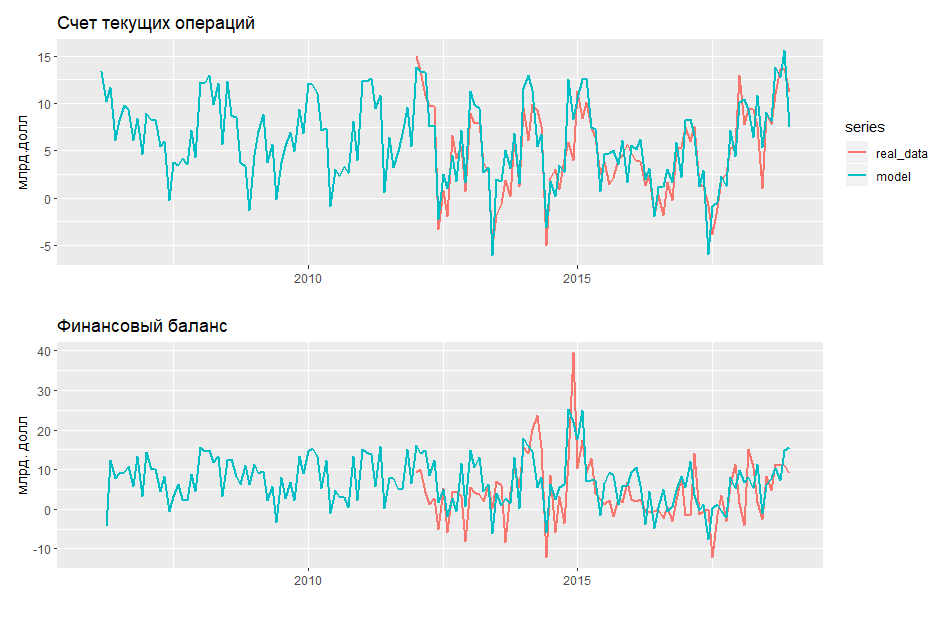
\includegraphics[width=10cm]{cur_fin.png}
\captionsetup{justification=centering,margin=0.5cm}
\caption{Модель платежного баланса: счет текущих операций и финансовый баланс}\label{fi:3}
\captionsetup{margin=0cm}
\end{figure}
\end{frame}

\begin{frame}
	\frametitle{Прогноз модели на тестовой выборке}
\begin{figure}[htp!]
	\centering
	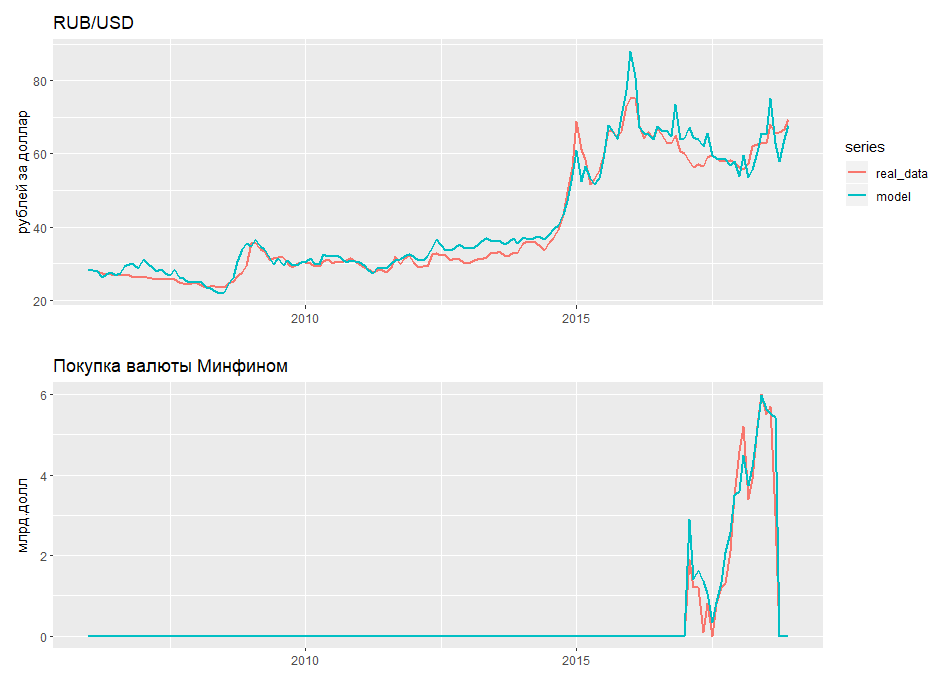
\includegraphics[width=9cm]{rub_purch.png}
	\caption{Модели обменного курса и покупки валюты}\label{fi:5}
	\captionsetup{justification = centering, margin=0cm}
\end{figure}

\end{frame}

\begin{frame}
	\frametitle{Прогноз модели на тестовой выборке}
\begin{figure}[htp!]
	\centering
	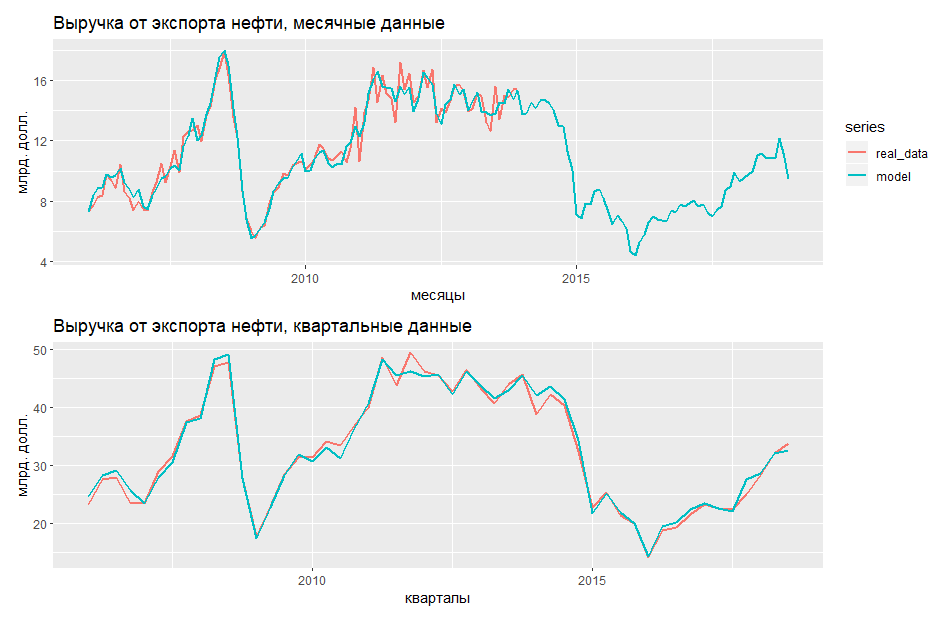
\includegraphics[width=10cm]{oil_rev.png}
	\caption{Выручка от экспорта нефти}\label{fi:5}
	\captionsetup{justification=centering,margin=0cm}
\end{figure}
\end{frame}

\begin{frame}
\frametitle{Сценарный анализ}
\begin{itemize}
		\item В работе построены сценарные прогнозы на 2020 год. 
		
		\item Рассмотрено три сценария:		
\begin{center}
	\footnotesize
	\begin{tabular}{c| c | c | c}
		Переменная & Базовый & Оптимистичный & Пессимистичный \\
		\toprule
		Brent & $33$ & $ 64.9$ & $27$ \\
		$\Delta$ ВВП &  $-5.5 \%$  & $0\%$ &  $-8\%$  \\
		Ключевая ставка &  $5.5 \%$ до $07.20$,  & $5.5 \%$ до $07.20$, &  $5.5 \%$\\
		&$5 \%$ до $12.20$ & $5 \%$ до $10.20$, $4.5 \%$ до $12.20$ & \\
		USD/EUR & $1.1$ & $1.2$ & $1.08$ \\
		Цена отсечения & $42.44$ & $42.44$ & $42.44$\\
		\bottomrule
	\end{tabular}
	\captionof{table}{Сценарии экзогенных переменных}\label{tab:7}
	\normalsize
\end{center}
		
\item Траектории остальных экзогенных переменных спрогнозированы с помощью сезонной наивной модели.
\end{itemize}
\end{frame}

\begin{frame}
	\frametitle{Сценарные прогнозы}
\begin{figure}[htp]
	\centering
	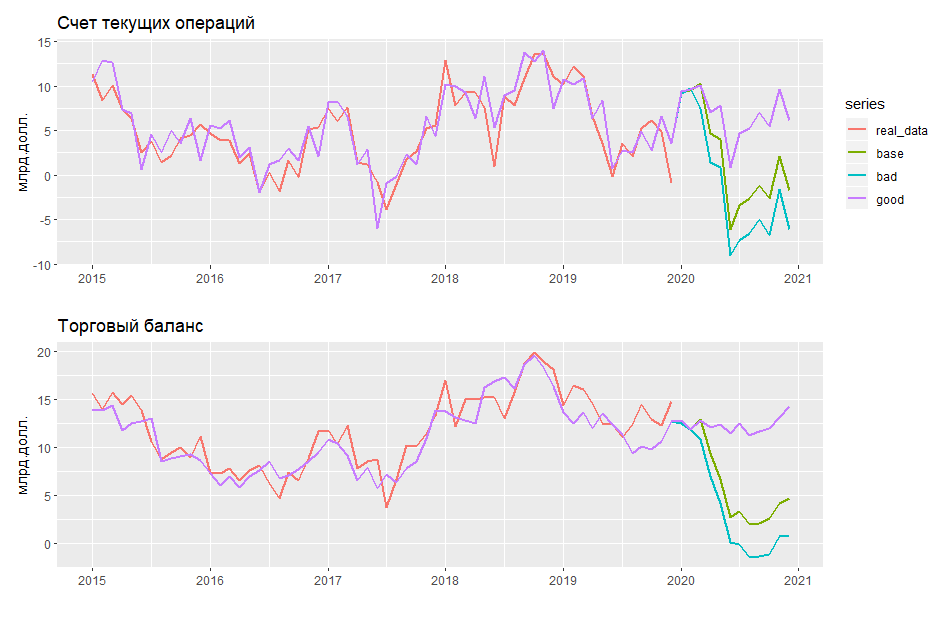
\includegraphics[width=10cm]{curtrade.png}
	\caption{Компоненты платежного баланса}\label{fi:7}
\end{figure}
\end{frame}

\begin{frame}
	\frametitle{Сценарные прогнозы}
\begin{figure}[htp]
	\centering
	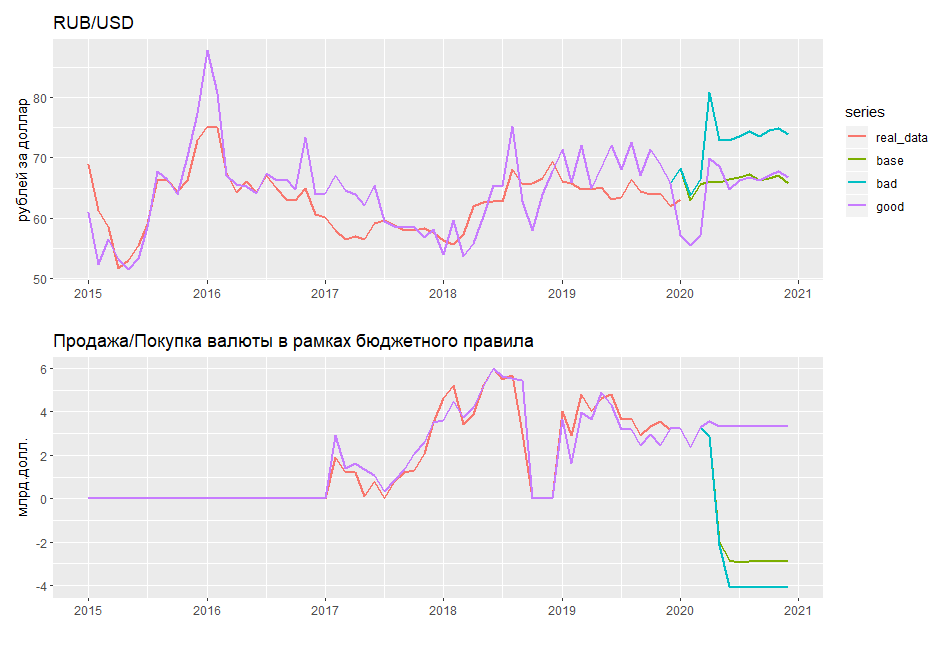
\includegraphics[width=10cm]{rub_2015.png}
	\caption{Валютный курс и покупка валюты Минфином}\label{fi:8}
\end{figure}
\end{frame}


\begin{frame}
		\frametitle{Выводы}
	\begin{itemize}
		\item Предложена модель внешнеэкономической деятельности РФ, включающая блок платежного баланса в разбивке на отдельные счета и их компоненты, уравнение валютного курса (RUB/USD), уравнение покупки валюты в рамках бюджетного правила и блок моделей топливных ресурсов.
		\item Построены прогнозы на $2020$ год при базовом, оптимистичном и пессимистичном сценариях.
		\item Прогнозы демонстрируют высокую зависимость устойчивости платежного баланса РФ (способности поддерживать профицит счета текущих операций) от цен на нефть. 
		В базовом и пессимистичном сценариях, при среднем
		уровне цен на нефть марки Brent ниже цены отсечения, на протяжении $2020$
		года ожидается дефицит счета текущих операций.
	\end{itemize}	
\end{frame}

\begin{frame}[c]
\begin{center}

{\LARGE Спасибо за внимание!}

\bigskip

{\insertauthor} 

\bigskip\bigskip


\bigskip\bigskip


\end{center}
\end{frame}

\begin{frame}
\frametitle{Приложение 1: эндогенные переменные}
\small
\begin{center}
	\begin{tabular}{ l | c }
		\toprule
		Эндогенные переменные  & Обозначение в модели  \\
		\midrule
		\multicolumn{2}{c}{Эконометрические соотношения}\\
		\midrule 
		экспорт прочих товаров & \textit{ r\_exp\_othg } \\
		экспорт услуг & \textit{ r\_exp\_serv } \\
		импорт товаров &  \textit{ r\_imp\_goods } \\  
		импорт услуг &  \textit{ r\_imp\_serv } \\  
		баланс оплаты труда &  \textit{ r\_bal\_wage } \\  
		баланс ренты и вторичных доходов &  \textit{ r\_bal\_rent\_sinc } \\ 
		баланс инвестиционных доходов &  \textit{ r\_bal\_inv } \\
		изменение резервных активов &  \textit{ dif\_reserves } \\
		чистые ошибки и пропуски &  \textit{ r\_errors } \\
		\bottomrule
		\end{tabular}

	\captionof{table}{Модель платежного баланса}\label{tab:2}
\end{center}

\end{frame}

\begin{frame}
	\frametitle{Приложение 2: эндогенные переменные}
	\small
	\begin{center}
		\begin{tabular}{ l | c }
			\toprule
			Эндогенные переменные  & Обозначение в модели  \\
			\midrule
		\multicolumn{2}{c}{Балансовые соотношения}\\
		\midrule
		экспорт товаров & \textit{ r\_exp\_goods } \\
		импорт  &  \textit{ r\_imp\_all } \\  
		экспорт  &  \textit{ r\_exp\_all } \\  
		торговый баланс  &  \textit{ r\_bal\_trade } \\
		баланс услуг  &  \textit{ r\_bal\_serv } \\
		счет текущих операций  &  \textit{ r\_cur\_account } \\
		финансовый баланс  &  \textit{ r\_bal\_fin } \\
		\bottomrule
	\end{tabular}
	
	\captionof{table}{Модель платежного баланса: продолжение}\label{tab:3}
\end{center}
\end{frame}


\begin{frame}
	\frametitle{Приложение 3: экзогенные переменные}
\begin{center}
	\small
	\begin{tabular}{ l | c }
		\toprule
		Экзогенные переменные  &  Обозначение в модели  \\
		\midrule
		\multicolumn{2}{c}{показатели мировых рынков}\\
		\midrule
		цена нефти марки Brent & brent \\
		цена природного газа, LNG & gas\_lng \\
		цена природного газа, Europe & gas\_europe \\
		курс USD/EUR & usd\_eur \\
		EM index & em\_index \\
		\midrule
		\multicolumn{2}{c}{показатели добычи и переработки}\\
		\midrule
		добыча нефти & v\_prod\_oil \\
		первичная переработка нефти & v\_prod\_op \\
		добыча природного газа & v\_prod\_gas \\
		\bottomrule			
	\end{tabular}
	\captionof{table}{Экзогенные переменные}\label{tab:4} 
	\normalsize
\end{center}
\end{frame}



\begin{frame}
	\frametitle{Приложение 4: экзогенные переменные}
	\begin{center}
		\small
		\begin{tabular}{ l | c }
			\toprule
			Экзогенные переменные  &  Обозначение в модели  \\
			\midrule
			\multicolumn{2}{c}{показатели денежно-кредитной политики}\\
			\midrule
			ставка РЕПО, \% & rate\_repo \\ 
			доходность 10Y Treasury, \% & rate\_10tr \\
			ширина валютного коридора & vcor \\		
			цена отсечения по валютному правилу & r\_price\_cur\_purch\\
			\midrule	
			\multicolumn{2}{c}{ВПП и показатели внутреннего спроса}\\
			\midrule
			ВВП, номиналный & n\_y \\ 
			потребление домашних хозяйств & n\_c \\ 
			потребление государства & n\_g \\
			ВНОК & n\_j  \\ 
			Изменение запасов & n\_ds \\
			\bottomrule			
		\end{tabular}
		\captionof{table}{Экзогенные переменные: продолжение}\label{tab:5} 
		\normalsize
	\end{center}
\end{frame}


\begin{frame}
	\frametitle{Приложение 5: модель покупки валюты}
\begin{align*}
\text{r\_cur\_}&\text{purch}_t = \text{r\_dum\_cur\_purch}_t \cdot (c_1 \cdot \text{r\_cur\_purch}_{t-1} + \\
& + \quad c_2 \cdot \text{r\_price\_cur\_purch}_t + \lsum_{i=0}^2 c_{i+3} \cdot \text{brent}_{t-i}) + \varepsilon_{t},
\end{align*}
где $\text{r\_dum\_cur\_purch}_t$ — дамми-переменная, равная единице в период $t$, когда Минфин выходил на валютный рынок.
\end{frame}


\begin{frame}
	\frametitle{Приложение 6: модели нефти и газа}
	\footnotesize
	\textit{Модель газа:}
	\begin{align*} 
	\begin{cases}
	\text{p\_exp\_gas}_t =&c_1 + \text{dum\_2012}_t {+} \lsum_{i = 1,3,5,6}b_{i} \cdot \text{brent}_{t-i} + \lsum_{i = 3, 5} g_i \cdot \text{gas\_lng}_{t-i} + \\ 
	&+ \quad c_2 \cdot \text{gas\_europe}_t + \varepsilon_{t,p} \\
	\text{v\_exp\_gas}_t =&\lsum_{j = 1}^{11} d_j \cdot \text{dum}_{jt} \cdot(a_1 + a_2 \cdot \text{v\_prod\_gas}_{t} + a_3 \cdot \text{usd\_eur}_{t} + \\ 
	&+ \quad a_4 \cdot \frac{\Delta\text{usd\_rub}_{t-1}}{\text{usd\_rub}_{t-2}} +
	\lsum_{i = 1, 7} p_i \cdot \widehat{ \text{p\_exp\_gas}}_{t-i})+  \varepsilon_{t,v}\\
	\text{r\_exp\_gas}_t =&\text{p\_exp\_gas}_t \cdot \text{v\_exp\_gas}_t + \varepsilon_{t,r}
	\end{cases}
	\end{align*}
	
	\vspace{5mm}
	
	\textit{Модель нефтепродуктов:}
	\begin{align*} 
	\begin{cases}
	\text{p\_exp\_op}_t =&c_1 + \lsum_{i = 0}^{3}c_{2 + i} \cdot \text{brent}_{t-i} + \varepsilon_{t,p} \\
	\text{v\_exp\_op}_t =&\lsum_{j = 1}^{11} d_j \cdot \text{dum}_{jt} \cdot (a_1 + a_2 \cdot \text{v\_prod\_op}_{t-1} + a_3 \cdot \frac{\text{usd\_rub}_{t-1}}{\text{usd\_rub}_{t-2}} + \\  
	&+ \quad a_4 \cdot \widehat{ \text{p\_exp\_op}_{t-1}}) + \varepsilon_{t,v} \\
	\text{r\_exp\_op}_t =&\text{p\_exp\_op}_t \cdot \text{v\_exp\_op}_t + \varepsilon_{t,r}
	\end{cases}
	\end{align*}
\end{frame}



\begin{frame}
	\frametitle{Приложение 7: модель платежного баланса (1)}
	\footnotesize
	\begin{itemize}
		\item Экспорт
		
		Первый шаг:
		\begin{align*}
		\begin{cases}        
		\text{r\_exp\_othg}_t =& \lsum_{j = 1}^{11} d_j \cdot \text{dum}_{jt} \cdot (c_1 +
		(c_2 \cdot \widehat{\text{r\_exp\_fuels}}_t +  \\
		& + c_3 \cdot \text{dum\_1114}_t \cdot \widehat{\text{r\_exp\_fuels}}_t) + 
		\varepsilon_{t, othg} \\
		\text{r\_exp\_goods}_t =& \widehat{\text{r\_exp\_fuels}}_t + \widehat{\text{r\_exp\_othg}}_t + \varepsilon_{t, gds},
		\end{cases}
		\end{align*}
		где 
		\[
		\widehat{\text{r\_exp\_othg}}_t =\widehat{\text{r\_exp\_oil}}_t + \widehat{\text{r\_exp\_op}}_t + \widehat{\text{r\_exp\_gas}}_t.
		\]
		
		Второй шаг:
		\begin{align*}	
		\begin{cases}        
		\text{r\_exp\_serv}_t =& \lsum_{j = 1}^{11} d_j \cdot \text{dum}_t \cdot (c_1 + c_2 \cdot \widehat{\text{r\_exp\_goods}}_t + \\ &
		+ \quad c_3 \cdot \widehat{\text{r\_imp\_serv}}_t) + \varepsilon_{t, srv}\\
		\text{r\_bal\_trade}_t =& \widehat{\text{r\_exp\_goods}}_t - \widehat{\text{r\_imp\_goods}}_t + \varepsilon_{t, bt}\\
		\text{r\_bal\_serv}_t =& \widehat{\text{r\_exp\_serv}}_t - \widehat{\text{r\_imp\_serv}}_t + \varepsilon_{t, bs}
		\end{cases}
		\end{align*}

	\end{itemize}
\end{frame}

\begin{frame}
	\frametitle{Приложение 8: модель платежного баланса (2)}
	\footnotesize
	\begin{itemize}
		
		\item Импорт
		
		\begin{align*}
		\begin{cases}        
		\text{r\_imp\_goods}_t =& \lsum_{j = 1}^{11} d_j \cdot \text{dum}_{jt} \cdot (c_1 +
		\frac{c_2\cdot\text{n\_c}_{t-1} +
			c_3\cdot\text{n\_j}_{t-1} +
			c_4\cdot\text{n\_ds}_{t-1}}{\text{usd\_rub}_{t-1}}) + \\  
		& + \quad c_5 \cdot \widehat{\text{r\_exp\_goods}}_{t-1} + \varepsilon_{t, gds} \\
		\text{r\_imp\_serv}_t =& \lsum_{j = 1}^{11} \rho_j \cdot \text{dum}_t \cdot (a_1 +
		\frac{a_2 \cdot \text{n\_c}_{t-1} +
			a_3 \cdot \text{n\_j}_{t-1} +
			a_4  \cdot \text{n\_ds}_{t-1}}{\text{usd\_rub}_{t-1}} + \\  
		&+ \quad a_5 \cdot \widehat{\text{r\_imp\_goods}}_{t-1} + \varepsilon_{t, srv} \\
		\text{r\_imp\_all}_t =& \widehat{\text{r\_imp\_goods}}_t + \widehat{\text{r\_imp\_serv}}_t + \varepsilon_{t, all}
		\end{cases}
		\end{align*}
		
		\item Баланс оплаты труда
		
		
		\begin{align*}
		\text{r\_bal}\text{\_wage}_t =& \lsum_{j = 1}^{11} d_j \cdot \text{dum}_{jt} \cdot (c_1 + 
		c_2 \cdot \widehat{ \text{r\_exp\_oil}}_t + c_3 \cdot \widehat{ \text{r\_exp\_othg}}_t + \\
		& + \quad c_4 \cdot \widehat{ \text{r\_exp\_serv}}_t + c_5 \cdot \widehat{ \text{r\_imp\_serv}}_t) + \varepsilon_{t, bw} 
		\end{align*}
		
		\item Баланс ренты и вторичных доходов
		
		\begin{align*}
		\text{r\_rent\_sinc}_t = & \lsum_{j = 1}^{11} d_j \cdot \text{dum}_t \cdot (c_1 + c_2 \cdot \widehat{ \text{r\_exp\_goods}}_t + \\
		& c_3 \cdot \widehat{ \text{r\_exp\_serv}}_t) + \varepsilon_{t, rs} 
		\end{align*} 
		
		\item Баланс инвестиционных доходов
		
		\begin{align*}
		\begin{cases}
		\text{r\_bal\_inv}_t =& \lsum_{j = 1}^{11} d_j \cdot \text{dum}_t \cdot (c_1 + c_2 \cdot \widehat{\text{r\_bal\_trade}}_t + \\
		& + \quad c_3 \cdot \widehat{\text{r\_bal\_serv}}_t) + \varepsilon_{t, bi} \\ 
		\text{r\_cur\_acc}_t =& \widehat{\text{r\_bal\_inv}}_t + \widehat{ \text{r\_bal\_rent\_sinc}}_t + \widehat{\text{r\_bal\_wage}}_t +\\ & + \quad \widehat{\text{r\_bal\_serv}}_t +
		\widehat{\text{r\_bal\_trade}}_t + \varepsilon_{t, ca} 
		\end{cases}
		\end{align*} 
	\end{itemize}
\end{frame}

\begin{frame}
	\frametitle{Приложение 9: модель платежного баланса (3)}
	\footnotesize
	\begin{itemize}		
		\item Баланс инвестиционных доходов
		
		\begin{align*}
		\begin{cases}
		\text{r\_bal\_inv}_t =& \lsum_{j = 1}^{11} d_j \cdot \text{dum}_t \cdot (c_1 + c_2 \cdot \widehat{\text{r\_bal\_trade}}_t + \\
		& + \quad c_3 \cdot \widehat{\text{r\_bal\_serv}}_t) + \varepsilon_{t, bi} \\ 
		\text{r\_cur\_acc}_t =& \widehat{\text{r\_bal\_inv}}_t + \widehat{ \text{r\_bal\_rent\_sinc}}_t + \widehat{\text{r\_bal\_wage}}_t +\\ & + \quad \widehat{\text{r\_bal\_serv}}_t +
		\widehat{\text{r\_bal\_trade}}_t + \varepsilon_{t, ca} 
		\end{cases}
		\end{align*} 
		
		\item Финансовый баланс
		
		\[
		\widehat{\text{r\_bal\_fin}}_t = \widehat{\text{r\_cur\_acc}}_t + \widehat{\text{r\_errors}}_t - \widehat{\text{dif\_res}}_t
		\]
		

		\item Чистые ошибки и пропуски
		
		\begin{align*}
		\text{r\_errors}_t = c_1 + c_2\cdot \Delta \text{brent}_t  + \lsum_{j = 1}^{11} d_j \cdot \text{dum}_t
		\end{align*}
	\end{itemize}
\end{frame}

\begin{frame}
\frametitle{Приложение 10: метрики качества (1)}	
	\begin{center}
		\footnotesize
		\begin{tabular}{l|rr|rr|rr|rr}
			\toprule
			\multirow{2}{*}{series}&\multicolumn{2}{c|}{\textbf{bp\_model}}&\multicolumn{2}{c|}{\textbf{arima}}&\multicolumn{2}{c|}{\textbf{ets}}&\multicolumn{2}{c}{\textbf{snaive}}\\
			
			&MAPE & MASE & MAPE & MASE & MAPE & MASE & MAPE & MASE \\ 
			\midrule
			p\_exp\_gas & \textbf{0.02} & 1.93 & 0.05 & 2.22 & 0.06 & 2.37 & 0.03 & \textbf{1.16} \\ 
			p\_exp\_oil & \textbf{0.01} & \textbf{0.43} & 0.04 & 1.54 & 0.04 & 1.63 & 0.04 & 1.72 \\ 
			p\_exp\_op & \textbf{0.02} & \textbf{0.91} & 0.08 & 5.07 & \textbf{0.02} & 1.52 & 0.04 & 2.54 \\ 
			r\_bal\_fin & \textbf{1.61} & \textbf{0.96} & 2.73 & 1.07 & 4.35 & 1.39 & 3.37 & 1.63 \\ 
			r\_bal\_inv & 0.36 & 1.09 & \textbf{0.28} & \textbf{0.52} & 0.29 & 0.56 & 0.33 & 0.63 \\ 
			r\_bal\_rent\_sinc & \textbf{0.44} & 2.02 & 0.55 & 0.77 & 0.58 & 0.84 & 0.49 & \textbf{0.73} \\ 
			r\_bal\_serv & 2.14 & 1.21 & 0.26 & 1.26 & \textbf{0.13} & 0.62 & 0.22 & \textbf{1.06} \\ 
			r\_bal\_trade & 0.17 & 1.72 & \textbf{0.14} & \textbf{1.31} & 0.35 & 3.26 & 0.25 & 2.39 \\ 
			r\_bal\_wage & 0.25 & \textbf{1.53} & 0.33 & 4.35 & 0.35 & 5.04 & \textbf{0.17} & 3.21 \\ 
			r\_cur\_account & \textbf{0.36} & \textbf{1.63} & 5.83 & 2.86 & 4.36 & 2.31 & 2.49 & 1.84 \\ 
			r\_cur\_purch & \textbf{0.20} & \textbf{0.59} & 1.13 & 6.03 & 1.00 & 5.43 & 0.48 & 2.41 \\ 
			r\_dif\_reserves & 1.28 & \textbf{1.11} & 0.82 & 1.48 & \textbf{0.59} & 1.16 & 1.19 & 1.68 \\ 
			r\_errors & 1.90 & 0.95 & 1.11 & 0.67 & \textbf{1.03} & \textbf{0.61} & 1.86 & 0.88 \\ 
			r\_exp\_all & \textbf{0.05} & \textbf{0.90} & 0.08 & 1.53 & 0.06 & 1.09 & 0.07 & 1.40 \\ 
			\bottomrule
		\end{tabular}
		\captionsetup{justification=centering,margin=2cm}
		\captionof{table}{Метрики качества для модели внешнеэкономической деятельности и бенчмарков}\label{tab:4}
	\end{center}

\end{frame}

\begin{frame}
	\frametitle{Приложение 11: метрики качества (2)}	
\begin{center}
		\footnotesize
		\begin{tabular}{l|rr|rr|rr|rr}
			\toprule
			\multirow{2}{*}{series}&\multicolumn{2}{c|}{\textbf{bp\_model}}&\multicolumn{2}{c|}{\textbf{arima}}&\multicolumn{2}{c|}{\textbf{ets}}&\multicolumn{2}{c}{\textbf{snaive}}\\
			
			&MAPE & MASE & MAPE & MASE & MAPE & MASE & MAPE & MASE \\ 
			\midrule
	r\_exp\_gas & \textbf{0.08} & 0.88 & 0.12 & 1.05 & 0.09 & \textbf{0.73} & 0.14 & 1.22 \\ 
	r\_exp\_goods & \textbf{0.03} & \textbf{0.54} & 0.09 & 1.69 & 0.07 & 1.40 & 0.08 & 1.53 \\ 
	r\_exp\_oil &\textbf{0.04} & 0.90 & 0.07 & \textbf{0.87} & 0.07 & 0.90 & 0.07 & 0.91 \\ 
	r\_exp\_op & \textbf{0.08} & 0.87 & 0.09 & \textbf{0.65} & 0.12 & 0.81 & 0.11 & 0.79 \\ 
	r\_exp\_othg & 0.05 & \textbf{0.49} & 0.05 & 0.79 & \textbf{0.04} & 0.70 & 0.06 & 0.91 \\ 
	r\_exp\_serv & 0.19 & 1.16 & 0.05 & \textbf{0.47} & \textbf{0.04} & 0.42 & 0.06 & 0.60 \\ 
	r\_imp\_all & \textbf{0.04} & \textbf{0.35} & 0.07 & 1.02 & 0.07 & 0.99 & 0.05 & 0.77 \\ 
	r\_imp\_goods & \textbf{0.04} & \textbf{0.37} & 0.06 & 0.88 & 0.09 & 1.29 & 0.05 & 0.81 \\ 
	r\_imp\_serv & 0.16 & 1.31 & 0.08 & 0.82 & \textbf{0.04} & \textbf{0.34} & 0.06 & 0.61 \\ 
	rub\_usd & \textbf{0.06} & \textbf{1.61} & 0.11 & 6.37 & 0.13 & 7.75 & \textbf{0.06} & 3.63 \\ 
	v\_exp\_gas & \textbf{0.08} & \textbf{0.84} & 0.14 & 1.36 & 0.09 & 0.92 & 0.14 & 1.36 \\ 
	v\_exp\_oil & \textbf{0.04} & 1.09 & 0.05 & 0.74 & 0.05 & \textbf{0.72} & \textbf{0.04} & 0.61 \\ 
	v\_exp\_op & \textbf{0.08} & 0.95 & 0.10 & \textbf{0.74} & 0.10 & 0.76 & 0.11 & 0.84 \\ 
	\bottomrule
	\end{tabular}
	\captionsetup{justification=centering,margin=2cm}
	\captionof{table}{Метрики качества для модели внешнеэкономической деятельности и бенчмарков}\label{tab:5}
	\end{center}
\end{frame}

\begin{frame}
	\frametitle{Приложение 12: сценарные прогнозы выручки нефти и газа}
	\begin{figure}[htp]
		\centering
		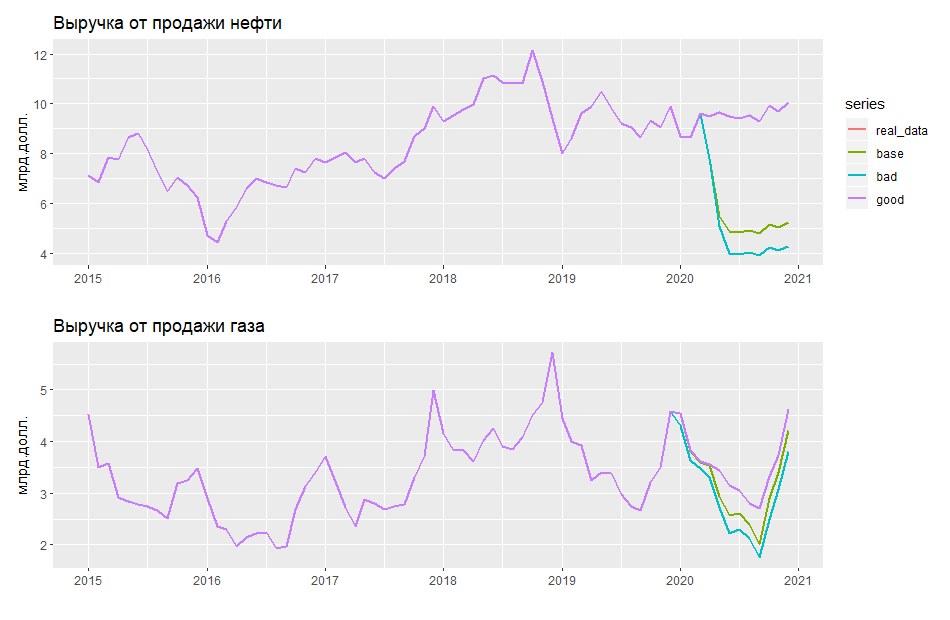
\includegraphics[width=10cm]{oil_2015.png}
		\caption{Выручка от экспорта нефти и газа}\label{fi:9}
	\end{figure}
\end{frame}

\end{document}